\documentclass{article}


\usepackage[ngerman]{babel}
\usepackage[T1]{fontenc}    
\usepackage[utf8]{inputenc}
\usepackage{newspaper}
\usepackage{times}
\usepackage{graphicx}
\usepackage{multicol}

\usepackage{wrapfig}

\usepackage{picinpar}
%uasage of picinpar:
%\begin{window}[1,l,\includegraphics{},caption]xxxxx\end{window}

%%%%%%%%%  Front matter   %%%%%%%%%%

\date{\today}
\currentvolume{1}
\currentissue{2}
\SetPaperName{Model Based Times}
\SetHeaderName{Model Based Times}
\SetPaperLocation{Braunschweig}
\SetPaperSlogan{\textbf{Gruppe 007:} \\
	Sofia Ananieva \\ Florian Maurer \\Stefan Mühlbauer \\ Julian Troegel}
\SetPaperPrice{5 CP}

\begin{document}
\maketitle

\begin{multicols}{3}{
		\headline{\it\huge Problem}
		User haben häufig Newsfeeds unterschiedlicher Formate und aus verschiedenen Quellen (RSS, Atom, …) abonniert. Dabei ist schwierig, sich einen schnellen und guten Überblick zu verschaffen. 
		\closearticle
		
		\headline{\it\huge Idea}
		RSS und Atom Feeds zusammentragen und in einen  LaTeX Zeitungsartikel umwandeln. Dazu müssen RSS und Atom Feeds in ein gemeinsames Metamodel gebracht werden. Aus dem gemeinsamen Metamodel werden die Artikel erstellt. Das gewünschte Layout wird durch ein Metamodel festgelegt und mit Constraints versehen. Evtl. können die Feeds mit weiteren Informationen angereichert werden (Volltext, Bilder, Personen, Orte usw. identifizieren)
		\closearticle
		
		\headline{\it\huge Benefit}
		Einen nostalgischen Überblick über aktuelle Themen geben. Man kann Newsfeeds als hübsche Zeitungsartikel konsumieren. Optional werden Artikel automatisch mit passenden Bildern oder auch Kartenausschnitten erweitert. 
		\closearticle
		
		\headline{\it\huge Action}
		\begin{itemize}
			\item RSS und Atom in ein unifiziertes Metamodel bringen
			\item Ggf. Metamodel anreichern (Volltext, Bilder, Clustering, …)
			\item Metamodel für das Layout erstellen und dafür Constraints  einbinden, z.B. geeignete Darstellungsweisen finden (Anzahl Spalten, Schriftgröße, farbliche Markierungen, Format usw.)\\
			Beispiele:
			\begin{itemize}
				\item Position \& Größenbereich von Bildern
				\item Anzahl Spalten, abhängig vom Format (DIN A4/DIN A3/\ldots)
				\item Schriftgröße
				\item Anzahl Zeichen für Titel \& Untertitel
				\item Volltext hat mindestens\ \ldots\ und maximal\ \ldots\ Zeichen
				\item Constraints reagieren dynamisch aufeinander, zum Beispiel: kleinere Schriftgröße erlaubt längere Artikel
			\end{itemize}
			\item Erstellung und Verwaltung von Artikel mittels DSL
			\begin{itemize}
				\item Zeitung erstellen können, ohne \LaTeX\ können zu müssen
				\item Manuell Artikel erstellen und in die Zeitung einbinden können
				\item Optionen zur Generierung der Zeitungsartikel 
			\end{itemize}
			\item Export des Layout Metamodels mittels LaTeX Template
		\end{itemize}
		
		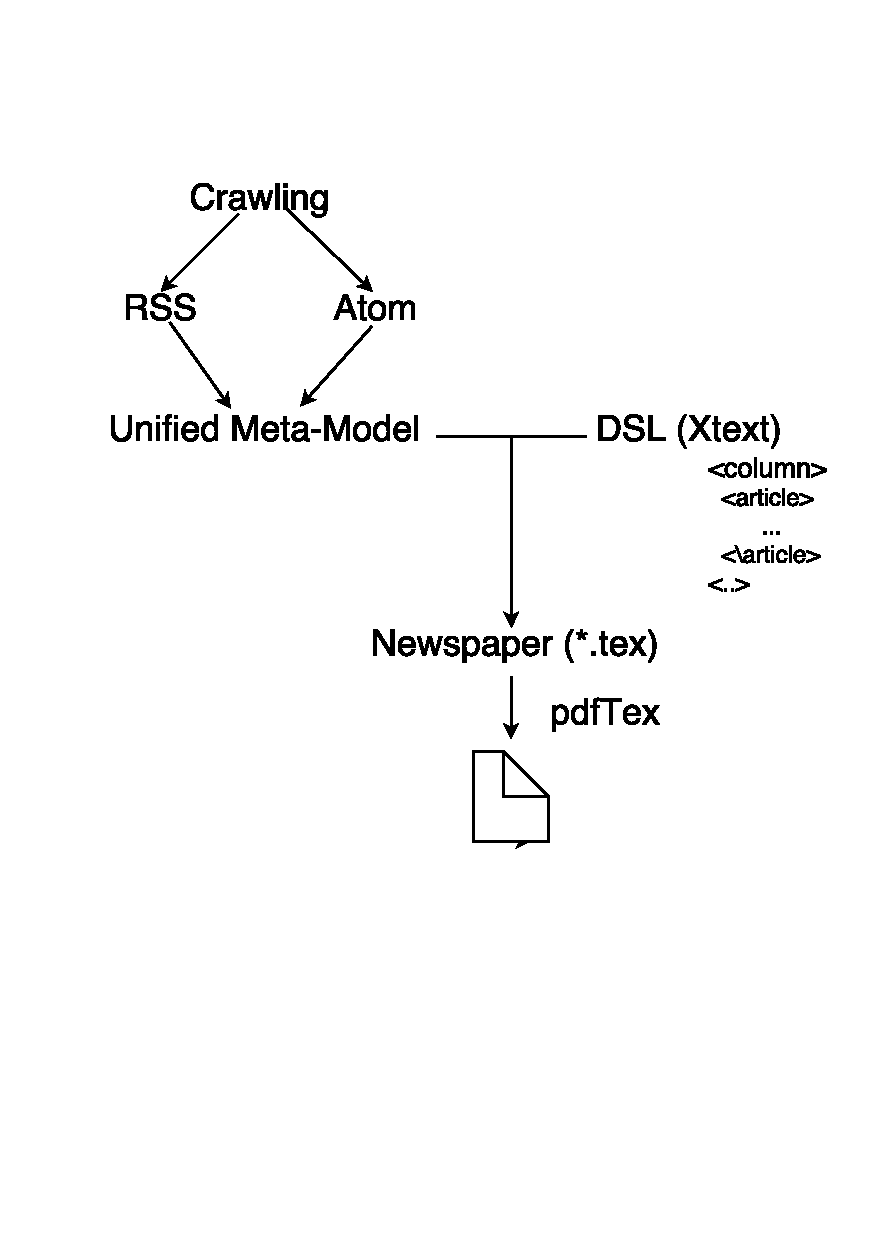
\includegraphics[trim=0 180 0 80,clip,width=\columnwidth]{modelbasedtimesDiagram.pdf}
		\centerline{Ein möglicher Diagrammablauf}
		\closearticle
		
		\headline{\it\huge Technologien}
		\begin{itemize}
			\item RSS
			\item Atom
			\item Ecore
			\item OCL
			\item Xtext
			\item \LaTeX\ Compiler
			\item evtl. Google Maps
		\end{itemize}
		\closearticle
		}

%\byline{\sc\Large Geek Designs New \LaTeX{} Package}{Matthew Allen}
%
%The package is basically a redefinition of the \verb+\maketitle+ command.  The model was the New York Times---hopefully I haven't violated any copyright laws.  I also had to redefine the plain pagestyle.  It kept me busy for a few nights after work.  The rest is packages other people have written.      
%
%\begin{window}[2,r,\includegraphics[width=1.0in]{Bilder/5minuten},\centerline{The Atom}] The \verb+multicols+ package allows using multiple columns without starting a new page.  Using floats is not possible in a columns environment, however with the \verb+picinpar+ package, I can set a picture inside a block of text---just like you one you see here.  Isn't \LaTeX{} cool?
%And now we're just filling more space, and yet more space.  
%\end{window}
%\closearticle
%
%
%\headline{\it\huge Another Headline}
%This is just an example to fill up some space, but as long as I have your attention, I'll give some newspaper advice.
%
%It's good to use different fonts for each headline.  This particular font was accomplished with the command \verb+\headline{\it\huge Another Headline}+.  The headline in the preceding article was accomplished with the command \verb+\byline{\sc\Large Geek Designs New \LaTeX{} Package}{Matthew Allen}+.
%
%Of course the commands don't look so nice when they're set in column format.  Look at the example file if you have any questions as to how this example was created.
%
%I suppose we could also show how an equation is type set:
%\begin{displaymath}
%x=\frac{-b\pm\sqrt{b^2-4ac}}{2a}
%\end{displaymath}
%and there you have it.  \closearticle
%}
\end{multicols}

\end{document}